\documentclass[10pt]{article} 
\usepackage[russian]{babel} % Required for inserting images 
\usepackage{graphicx} 
\usepackage{letterspace}
\usepackage[a5paper, top=1.5cm, bottom=1.5cm, left=1.5cm, right=1.5cm]{geometry} 
\usepackage{wrapfig}
\begin{document} 
\noindent легко устанавливается из правил дифференцирования, но мы не будем специально следить за этим, чтобы не удлинять изложение.

\textls[300]{Пример 1}. Равномерное движение: 

\begin{center} 
    \begin{math} 
        z(t)=z_0+vt. 
    \end{math} 
\end{center} 
Тогда \begin{math} z^{'}(t)=v \end{math} — постоянная величина. 
 
\textls[300]{Пример 2}. Равноускоренное движение: 
\begin{center} 
    \begin{math} 
        z=z_0+v_0 t+\frac{at^2}{2},  
    \end{math} 
\end{center} 
 
\noindent здесь \begin{math} v_0 \end{math} — начальная скорость, \begin{math} a \end{math} —ускорение. В этом случае \begin{math} z^{'}(t)=v_0+at \end{math} по известным правилам дифференцирования. Напомним, что если даны две функции  \begin{math} f(t), g(t) \end{math} и постоянная \begin{math} a, \end{math} то 
\begin{math} 
(f+g)^{'} = f^{'}+g^{'}, (af)^{'} = af^{'}, (fg)^{'} = f^{'}g+fg{'}, (\frac{f}{g})^{'} = \frac{f^{'}g-fg^{'}}{g^{2}} 
\end{math} (последняя формула верна в случае, когда \begin{math} g(t)\neq0 \end{math} в рассматриваемой точке t). Из предпоследней формулы следует, что \begin{math} (t^{2})^{'}=2t.\end{math}

При любом целом \begin{math} n \end{math} легко доказать (например, индукцией по \begin{math} n \end{math}), что \begin{math} (t^{n})^{'}=nt^{(n-1)}.\end{math} Можно доказать, что при \begin{math} t>0 \end{math} эта формула верна и для нецелых \begin{math} n \end{math} (об этом ещё будет идти речь ниже). 
 
Укажем геометрический смысл производной: если нарисовать график функции \begin{math} z=z(t),\end{math} то \begin{math} z^{'}=\tg\alpha \end{math}, где \begin{math} \alpha \end{math} — угол наклона касательной, проведённой к графику в точке \begin{math} (t, z(t)), \end{math} к оси \begin{math} t \end{math}(рис. 1). 
 
\textls[250]{Правило дифференцирования сложной функции}: если даны две функции \begin{math} F(z) \end{math} и \begin{math} z(t), \end{math} то для функции \begin{math} g(t)=F(z(t)) \end{math} производную можно найти по формуле 
 
\begin{center} 
    \begin{math} 
        g^{'}(t) = (F(z(t)))^{'} = F^{'}(z(t))z^{'}(t) 
     \end{math} 
\end{center} 
 
\begin{flushleft} вытекающей из того, что \end{flushleft} 
 
\begin{center} 
    \begin{math} 
        g^{'}(t)=\lim_{\substack{\triangle t\rightarrow 0}} \frac{\triangle g}{\triangle t} = \lim_{\substack{\triangle t\rightarrow 0}} \frac{\triangle F(z(t))}{\triangle t} = \lim_{\substack{\triangle t\rightarrow 0}} (\frac{\triangle F}{\triangle z} \frac{\triangle z}{\triangle t}) = F^{'}(z(t))z^{'}(t), 
     \end{math} 
\end{center} 
(здесь использовалось, что если \begin{math}\triangle t \rightarrow 0,\end{math}то и \begin{math} \triangle z \rightarrow 0).\end{math} 
 
\textls[300]{Правило дифференцирования обратной функции}. Пусть функция \begin{math} z=f(t) \end{math} строго монотонна на отрезке\begin{math}[t_1, t_2] \end{math} и имеет производную в каждой точке этого отрезка. Строгая монотонность\begin{wrapfigure}{l}{0.35\textwidth}
  \centering
  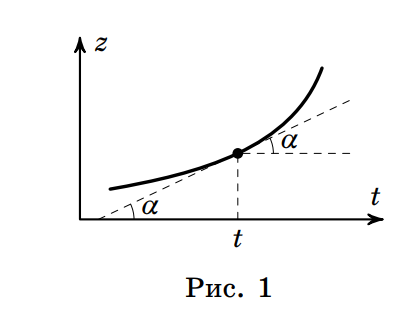
\includegraphics[width=0.35\textwidth]{Pic1.png}
\end{wrapfigure}
 означает, что функция \begin{math} f\end{math} либо возрастающая (если \begin{math} t^{'}<t^{''}, \end{math} то \begin{math} f(t^{'})< f(t^{''})), \end{math} либо убывающая (если \begin{math} t^{'}<t^{''}, \end{math} то \begin{math} f(t^{'})> f(t^{''})). \end{math} Будем для определённости считать функцию \begin{math} f \end{math} возрастающей. Тогда множество значений функции \begin{math} f \end{math} на отрезке\begin{math} [t_1,t_2] \end{math} представляет собой отрезок \begin{math} [z_1,z_2],\end{math} где \begin{math} z_1=f(t_1), z_2=f(t_2) \end{math} (рис. 2). При этом каждому значению \begin{math} z\in[z_1,z_2] \end{math} отвеча- 
\end{document}